\chapter{Solving Strategies}
\myTop{This chapter will present two different algorithms which can be used for solving a Rubik's Cube. These algorithms will be used as a foundation for the implementation part, which makes this chapter essential for the report.}
The two algorithms presented here are the beginners algorithm and Kociemba's optimal solver.
These two have been chosen because beginners algorithm is every inefficient with respect to the number of twist but can be performed quite simply \cite{beginner}, where Kociemba's is quite the opposite -- impossible to use for a human solver and extremely efficient with respect to the number of twists.
Because they are so different it will make a good foundation for the discussion later and this choice agrees with the problem limitations \ref{sec:problemLimitations}.

	\section{The Beginner's Algorithm}
\label{sec:beginner}
This section describes the easiest algorithm to remember for a human solver. The algorithm is divided into 5 different steps. Once the algorithm has been memorized, it is easy to recognize which step of the algorithm has been reached, so the correct move sequence can be applied. It is only necessary to remember a single move sequence for each step. The beginner's algorithm can however be made more efficient by remembering another somewhat similar move sequence for a few of the steps. Despite of this the beginner's algorithm is twist-wise quite inefficient, because purpose of the moves is to reach the next step instead of reaching the solved state and thereby taking a solving detour. 

\subsection{Step 1 - getting the cross}
The first step of the beginner's algorithm \cite{beginner} is to get a cross on any face. Getting a cross on a face means to align the \facelet{}s next to the center \facelet{}, so that all of the aligned \facelet{}s are of the same color, while at the same time the used edge pieces have the same color of the center \facelet{}s on each of the two faces on which they are.

\begin{wrapfigure}{R}{0.4\textwidth}
\begin{center}
	\includegraphics[width=0.35\textwidth]{input/pics/1FLCross.jpg}	
\end{center}
\caption{\myCaption{A first layer cross on the green face}}
\label{fig:1FL-cross}
\end{wrapfigure}

The face on which the cross is being assembled is set to be the top face. An edge piece that consists of the same colors as the center piece of the top face and the center piece of the front face is placed in the bottom of the front face. With two twists of the front face the edge piece is positioned correctly in the cross. If the edge piece is oriented correctly the cube is turned (noted y) and the process is repeated until the cross is assembled. However if the piece is oriented in the wrong way the following move sequence will change it's orientation without ruining any part of the cross that may already be assembled: \\

F' U L' U' or F U' R U

\subsection{Step 2 - completing the first layer}
When the cross is completed the next step is to position the corner pieces of the first layer correctly. The first layer is set as the down face (D). A corner with a \facet{} of the color of the down face is positioned directly above it's correct  position. The correct position is between the three faces that have the same colors as the three \facet{}s of the corner piece. Once the piece is above it's correct position, the cube should be viewed in such an angle that the piece is in the upper right corner of the front face, the following move sequence is repeated until the corner piece is oriented and positioned correctly: \\
%% Some thing is wrong in the part above, turn the cube around to have U facing down.

R' D' R D \\

If the piece is above the correct position the algorithm twists the corner clockwise and positions it in the correct position. If the piece is in the correct position the algorithm positions the piece above the correct position. The maximum number of repetitions until the piece is oriented and positioned correctly is five, because the piece can be two twists away from it's correct orientation. 
The move sequence can be performed inverted which twists the corner counterclockwise and looks as follows: \\

D' R' D R \\

If the correct move sequence is used the maximum number of repetitions is three. If number of twists and time used is not of importance it is only necessary to remember one of them.

\begin{wrapfigure}{R}{0.4\textwidth}
\begin{center}
	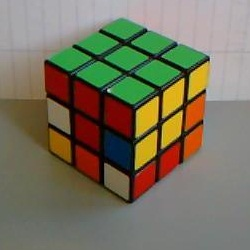
\includegraphics[width=0.35\textwidth]{input/pics/2FL.jpg}	
\end{center}
\caption{\myCaption{The first layer completed}}
\label{fig:2FL}
\end{wrapfigure}

\subsection{Step 3 - completing the second layer}
The purpose of this step is to position the four edges belonging to the second layer correctly. The move sequence used in this step either swaps the top edge piece of the front face with the left or right edge piece. That is why the edge piece that needs to be moved down to the second layer must be positioned at the top of the face that is next to the face of one of the edges colors, where the second color is the same as the front face's color. There is however a difference in which of the two faces is used as the front face, because if the wrong face is used as front face the piece will only be positioned correctly but not oriented correctly. That \facelet{} of the edge towards the front face must be of the same color as the front face. If the edge piece is to be swapped with the right edge piece of the front face the following move sequence is used: \\

U R U' R' U' F' U F \\

If the piece is to be swapped with the left edge piece of the front face the following move sequence is used: \\

U' L' U L U F U' F' \\

If none of the edge pieces who belong to the second layer are in the third layer and the first two layers is still not completed. This occurs if the edges are all in the second layer but not positioned or oriented correctly. One of the move sequences can be used to swap an edge piece from the third layer with one of the edges in the second layer which is not positioned or oriented correctly. Now the edge piece belonging to the second layer can be moved to it's correct position.

\begin{wrapfigure}[25]{R}{0.4\textwidth}
\begin{center}
	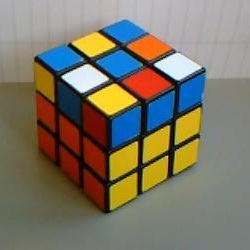
\includegraphics[width=0.35\textwidth]{input/pics/3F2L.jpg}	
\end{center}
\caption{\myCaption{The first two layers completed}}
\label{fig:3F2L}
\end{wrapfigure}

\subsection{Step 4 - getting the last layer cross}
%%%Step 4 is divided into 4 step? Perhaps substeps instead.
Solving the last layer is divided into four substeps. The order of these steps can be different and still yield the same result. We start out by getting the cross in the last layer, which is the same as the cross on the first layer. The move sequence used is however different. The only move sequence used in this step is the following: \\

F R U R' U' F' \\

Besides remembering the move sequence it is also important to know how the cube should be oriented.

If the up face colors form a line. The cube can be turned until the line forms a horizontal line. If the move sequence then is performed, the cross will be formed.

\begin{figure}[htb]
	\centering
		\subfloat[\myCaption{The up face colors form the opposite L.}]{\label{fig:cross:4LLcross1}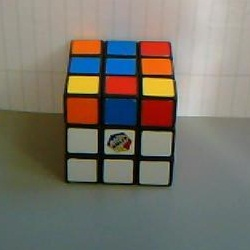
\includegraphics[width=0.28\textwidth]{input/pics/4LLcross1.jpg}}
		\hspace{0.02\textwidth}
		\subfloat[\myCaption{The up face colors form the horizontal line.}]{\label{fig:cross:5LLcross2}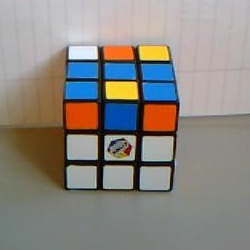
\includegraphics[width=0.28\textwidth]{input/pics/5LLcross2.jpg}}
		\hspace{0.02\textwidth}
		\subfloat[\myCaption{The up face colors form the cross.}]{\label{fig:cross:6LLcross3}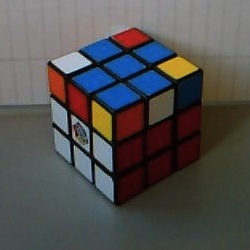
\includegraphics[width=0.28\textwidth]{input/pics/6LLcross3.jpg}}
		\caption{\myCaption{The steps in the completion of the last layer cross}}
		\label{fig:cross}
\end{figure}

If the up face colors form an opposite L character with the up face colors the move sequence will form the line. The cube must be oriented with the opposite L in the back left corner of the cube. 

If the up face colors do not form the opposite L the line or the cross, the move sequence will form the opposite L.

\begin{wrapfigure}{R}{0.4\textwidth}
\begin{center}
	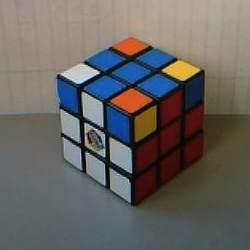
\includegraphics[width=0.35\textwidth]{input/pics/7LLedges.jpg}	
\end{center}
\caption{\myCaption{The correct oriented last layer cross.}}
\label{fig:7LLedges}
\end{wrapfigure}


To orient the cross correctly there is one move sequence to remember: \\

R U R' U R 2U R' \\

Again it is important to know how to orient the cube. By twisting the upper layer it is possible to position the upper layer so it either has two edge pieces next to each other or directly across from each other.

If the correct edges piece are next to each other. The cube must be oriented with a correct edge piece on the back face and a complete face on the right face. The move sequence will then make it possible to twist the up layer so that all the edge pieces are correctly positioned and oriented.

If the correct edge pieces are across each other the move sequence can be performed a single time to get two edge pieces next to each other.


\subsection{Step 5 - completing the last layer}
The purpose of this step is to position and orient the corners correctly. Firstly the corners must be positioned correctly. To do so there are two move sequences to remember -- one for rotating three corners clockwise and one for rotating them counterclockwise. It is however only necessary to remember one of them and repeat that one until the corners are positioned correctly, if the number of twists is unimportant to the solver. \\
\\
U R U' L' U R' U' L
\\
This move sequence will rotate the corners counterclockwise.
\\
\\
U' L' U R U' L U R'
\\
This move sequence will rotate the corners clockwise.
\\
\\
The orientation is again important to position the corners. If one of the corners already is positioned correctly. That corner is chosen not to be moved. 

If the three other corners need to be moved counterclockwise. The correct corner is positioned as the front right corner. The move sequence will then position the corners correctly.

If the three other corners need to be moved clockwise. The correct corner is positioned as the front left corner. The move sequence will then position the corners correctly.

If there are no correct corners. One of the two move sequences above performed once will make yield a correctly positioned corner.

\begin{wrapfigure}{R}{0.4\textwidth}
\begin{center}
	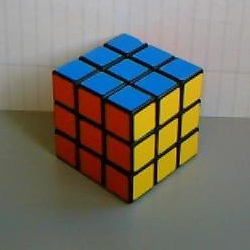
\includegraphics[width=0.35\textwidth]{input/pics/8done.jpg}	
\end{center}
\caption{\myCaption{The solved cube -- $e$}}
\label{fig:8done}
\end{wrapfigure}

To orient the corners correctly the move sequence from orienting the corners in the first layer is used: \\

R' D' R D \\

But in this step when one corner is completed. Instead of turning the whole cube to the next corner, the cube is locked on one face. Then when going to solve the next corner the upper layer is twisted until the incorrect corner is positioned at the front right corner of the cube and the move sequence is repeated.
	\section{Kociemba's Optimal Solver}
\label{sec:kociemba}
Kociemba's optimal solver is an algorithm created with the purpose of finding the twist-wise optimal solution to any scrambled \rubik{}\cite{kociemba09} \cite{cubelovers92}. It has been developed by Herbert Kociemba who has studied physics and mathematics at Technische Universit\"{a}t Darmstadt\cite{TUD} (1974-1979) and is currently teaching at a gymnasium. His interest in the \rubik{} started in the 1980 and he implemented his first algorithm -- Kociemba's Two Phase algorithm -- in 1990. See appendix  \ref{chap:emailCorrespondence} for the e-mail correspondence with Herbert Kociemba.

The Kociemba's optimal solver consists of two phases and is based on Kociemba's Two Phase algorithm. The first phase is based on a principle called relabeling, which will be defined at first. 

%In the following the Kociemba optimal solver will be described in detiail. Kociemba's Algorithm finds a solution to a scrambled \rubik{} using two phases and is based on another algorithm by Kociemba called Two Phase Algorithm. In order to fully understand kociemba's algorithm a process called relabeling must be defined at first.

\subsection{Relabeling}
The relabeling process  starts with choosing an up face with a corresponding down face. Then choosing a front face with a corresponding back face. Each \facelet{} with the color of the up or down face is marked with the letters ``UD''.  %Each edge \cpiece{} on the front and back where the \cpiece{} does not contain a ``UD'' sticker is marked with the letters ``FB''. 
Every edge \cpiece{} that is not labeled with "`UD"' is labeled with "`FB"' on the front and back face.
Figure \ref{fig:relabelClean} shows an example.
\begin{figure}[!hbt]
	\centering
		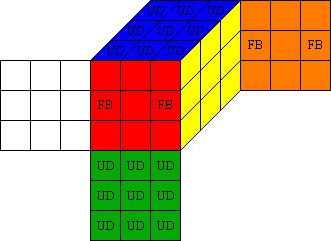
\includegraphics[scale = 0.8]{input/pics/relabelClean}
	\caption{\myCaption{A relabeled Rubik's Cube with the up and down faces as blue and green and red and orange as front and back.}}
	\label{fig:relabelClean}
\end{figure}
When relabeling a \rubik{} in the position $s$ it is written as $r(s)$. A \rubik{} in any position, $s$, is said to be in the set of positions called \m{H}(See subsection \ref{sub:theSubgroupH}) if and only if $r(s)=r(e)$.

\subsection{The subgroup H}
\label{sub:theSubgroupH}
%%% Beaware if the subgroup is introduced somewhere else. it should actually be. 
The moves \m{U}, \m{U'}, \m{U2}, \m{D}, \m{D'}, \m{D2}, \m{R2}, \m{L2}, \m{F2} and \m{B2} is the set of moves \m{A}. Using moves from \m{A} on a position in \m{H}, will always result in a \rubik{} in \m{H}. The reason for this can easily be tested with a \rubik{}. If using one of the three up face moves or one of the three down face moves, the ``FB'' labels are not moved and the ``UD'' labels are simply rotated on the face that is being twisted, see figure \ref{fig:relabel2:D}. The last four moves are all very similar to each other. If any side face -- not up or down -- is \twist{}ed 180 degrees, the three \facelet{}s on the up face is moved to the down face and vice versa and thereby keeping all the ``UD'' labels on the up and down face and keeping the orientation correct. The two remaining relabeled \facelet{}s are swapped which keeps the ``FB'' labels placed and oriented correctly, see figure \ref{fig:relabel2:R2}.


\begin{figure}[!hbt]
	\centering
	\subfloat[\myCaption{A relabeled cube that has been permutated with the move \m{D}.}]{\label{fig:relabel2:D}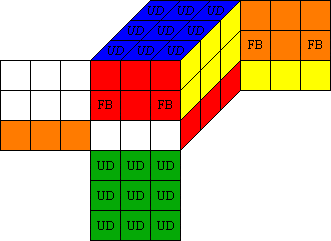
\includegraphics[width=0.45\textwidth]{input/pics/relabelD.PNG}}
	\hspace{0.05\textwidth}
	\subfloat[\myCaption{A relabeled cube that has been permutated with the move \m{R2}.}]{\label{fig:relabel2:R2}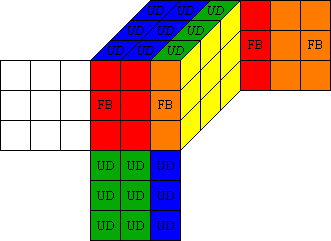
\includegraphics[width=0.45\textwidth]{input/pics/relabelR2.PNG}}
	\caption{\myCaption{Two positions which have been permuted with a move in \m{A}.}}
	\label{fig:relabel2}
\end{figure}

\subsection{Overall description}
\label{sub:overallDescription}
The first phase takes a scrambled cube $a$ and relabels it $r(a)$ then it finds a move sequence $b$ which will transform the relabeled cube into the subgroup \m{H}. This move will be denoted: $r(a)\cdot{}b \in \m{H}$. The second phase will then determine the length from the position $ab$ to the unit position $e$ by a table lookup. 


\begin{algorithm}[!h]                     
\caption{Kociemba's Algorithm \cite{rokicki09}}          
\label{alg:kociemba}        
\begin{algorithmic}[1]
\STATE $d=0$
\STATE {$l=\infty$}
\WHILE {$d<l$} 
	\FOR {$b \in S^{d}$}
		\IF {$r(ab) \in H$}
			\IF {$d + d_{2}(ab)<l$}
				\STATE {$l=d+d_{2}(ab)$}
			\ENDIF
		\ENDIF
	\ENDFOR
	\STATE {$d=d+1$}
\ENDWHILE
\STATE $l$ is now the length of the optimal solution to $a$
\end{algorithmic}
\end{algorithm}

The search distance in the algorithm ($d$), see figure \ref{fig:searchExpansion} is initially set to zero and the total length ($l$) is set to infinite. The total length is the amount of moves used to get from $a$ to $e$, while $d$ is the limited search length to find a move sequence that transforms the \rubik{} into a position in \m{H}. 
The \textbf{while} loop will run as long as $d$ is less than $l$.
%For the first run this is true, and will only test if the scrambled \rubik{} already is in the subgroup $H$. If so it will continue since a solution that goes out of $H$ might be a faster solution. 

The \textbf{for} loop runs through all move sequences in the range $d$ -- recall that $\m{S}^d$ is the set containing every move sequence that uses $d$ twists. This search of moves in $\m{S}^d$ is called the first phase and is further described in \ref{sub:firstPhase}.
Then an \textbf{if}-statement checks if the move sequence transforms the cube into the subgroup \m{H}. If so the algorithm checks whether $d + d_2(ab)$ is less than the length of the last solution, if so, $d + d_2(ab)$ is the new shortest move sequence, $l$, to $e$. 
The lookup table denoted $d_2(ab)$ returns the numbers of twist required to transform a position in \m{H} to the position $e$. This is done only by using moves in \m{A}. %$d_2(ab)$ is a lookup table which takes a position in $H$ and returns the number of twists it takes to transform the position to $e$ using moves in \m{A}
The lookup table is the second phase and is further described in the subsection \ref{sub:secondPhase}. 
The first time this \textbf{if}-statement is executed it will return true and this will be the new length of the solution. The \textbf{while} loop will end when $d$ is incremented to $l$, then the optimal solution has the length $l$. The actual solution is $b$ plus some move sequence in $\m{A}^{d_{2}(ab)}$. Figure \ref{fig:kociemba2} illustrates the algorithm.
\begin{figure}[!htb]
	\centering
	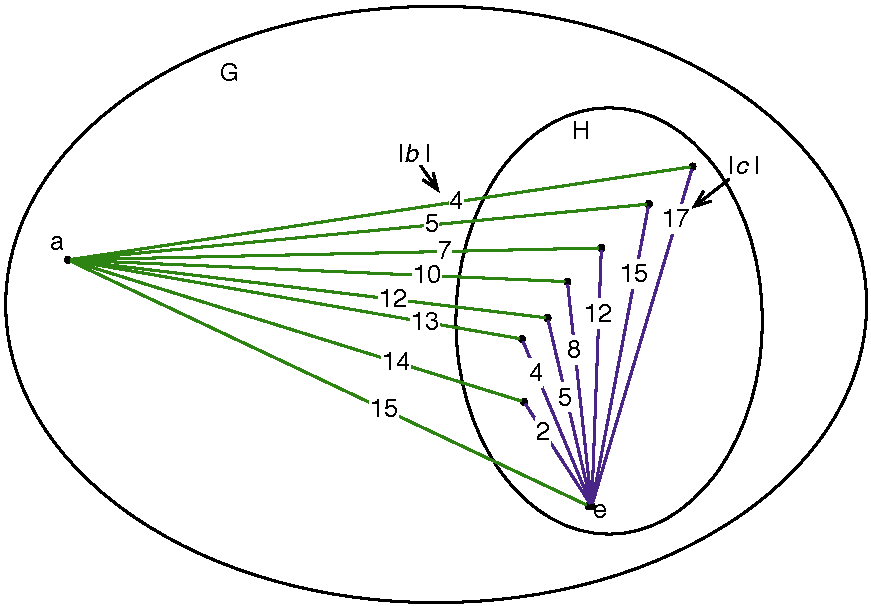
\includegraphics[scale=0.75]{input/pics/kocieambe2.pdf}
	\caption{\myCaption{The lines going from $a$ to a point in \m{H} is the move sequence denoted $b$. The lines from points in \m{H} to the point $e$ is the move sequence denoted $c$ . The numbers beside the lines are the number of moves. Note that the moves in $c$ is decreasing as the numbers of moves in $b$ is increasing. The line that goes directly from $a$ to $e$ is the shortest move sequence possible. }}
	\label{fig:kociemba2}
\end{figure}

\subsection{First phase}
\label{sub:firstPhase}
The first phase finds a move sequence, $b$, from a position $a$ that transforms the \rubik{} into the subgroup \m{H} this is done by going through all possible moves with a sequence of the length $d$. This is a breadth-first search algorithm \cite[pp. 729-731]{Rosen07}.
In figure \ref{fig:searchExpansion} the amount of elements in $\m{S}^d$ to a specific $d$ is illustrated.
An example of a search from a position $a$ is given. The algorithm starts by searching in $\m{S}^{d}$, where $d =  0$. This will give the position $a$ itself. The distance $d$ is then incremented to 1. This will result in 18 new possible move sequences all one twist away from $a$. Thereafter the $d$ is incremented and the search now moves 18 moves from the previous positions obtained in the search where $d = 1$. This allows a possibility for optimization of the algorithm since some of the moves will eventually be the same. e.g. the two move sequences R2 and R' R' is of length 1 and 2 respectively, but the result is the same transformed cube. The algorithm checks whether the transformed cube is in \m{H} by relabeling it and checking if $r(ab) = r(e)$. The actual implementation of the algorithm may vary and will be omitted for now.

$d$ continues to be incremented until it reaches the length $l$. Since $l$ starts with the value infinite, it has to be changed in order to stop the loop. This happens in the second phase.

\begin{figure}[!hbt]
	\centering
		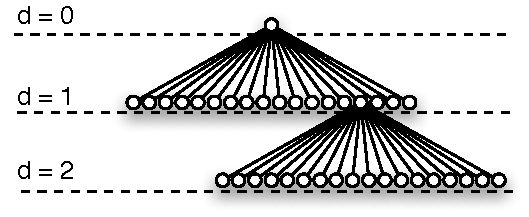
\includegraphics[scale=0.75]{input/pics/searchExpansion.pdf}
	\caption{\myCaption{As the distance of the search $d$ increases, the possible move sequences expands exponentially. For each vertex on the graph there is 18 child vertices. The amount of leaves for each search depth would be $18^{d}$.}}
	\label{fig:searchExpansion}
\end{figure}


\subsection{Second Phase}
\label{sub:secondPhase}
The goal of the second phase is to find the length of the shortest move sequence to transform the \rubik{} from a position in \m{H} to $e$. A way to solve this problem is by having a lookup table. This table has to be very large, considering the amount of positions in \m{H}. 

The amount of positions can be calculated by imagining that one were to assemble the \rubik{}, starting with a disassembled \rubik{}. The first corner \cpiece{} can be placed in eight different places. The next corner has seven possible positions etc. Note that all \cpiece{}s in a cube in \m{H} has the correct orientation. 
%until the last two corners which has a specific place since two corners can not be swapped. 
This gives $8! = 40320$ possibilities for the corners. 
The eight edges of the top and down layer can be placed similarly and also yields $8!$.  
The four edges of the middle layer can be placed in four different places this yield $4! = 24$. Since it is impossible to swap two corners without swapping any edges the amount of possibilities is halved. 
The final result is $\frac{4!\cdot(8!)^{2}}{2} \approx 19.508\cdot10^{9}$ elements in \m{H}.
The actual implementation of such a table will be discussed in chapter \ref{chap:kociembaImplement}.
\myTail{The two algorithms described in this chapter will be used in the implementation part. They have been chosen because of their differences.}